\section{Zielsetzung}
Ziel dieses Versuches ist es die Gültigkeit der Fourieranalyse und -synthese zu überprüfen.
Dafür werden versiedene periodische Signale in ihre Fourierkoeffizienten zerlegt.
Es wird überprüft ob es möglich ist die Signale aus den Koeffizienten zu rekonstruieren.
\section{Theorie}
\label{sec:Theorie}
Die wichtigsten periodischen Funktion sind die Sinus- und Cosinusfunktion.
Diese beiden sind $2\pi$ periodisch und besitzen einen Wertevorrat von $+1$ bis $-1$.
Mit ihnen ist es möglich fast jeden periodischen Vorgang zu beschreiben.
Dies lässt sich aus dem Fourierschen Theorem schließen.

\subsection{Das Fouriersche Theorem}
Sofern die Reihe
\begin{equation}
  \label{eq:gl1}
  \frac{a_0}{2}+\sum_{n=1}^\infty{(a_n\cos{\frac{2\pi}{T}t}+b_n\sin{\frac{2\pi}{T}t})}
\end{equation}
gleichmäßig konvergent ist, stellt diese eine periodische Funktion mit den Koeffizienten
\begin{equation}
  a_n=\frac{2}{T}\int_0^T f(t)\cos{n\frac{2\pi}{T}t}dt
\end{equation}
und
\begin{equation}
  b_n=\frac{2}{T}\int_0^T f(t)\sin{n\frac{2\pi}{T}t}dt
\end{equation}
dar.
In der Fourierentwicklung kommen nur ganzzahlige Vielfache der Grundfrequenz vor.
Diese nennt man harmonische Oberschwingungen.
Die ermittlung dieser Amplituden, also der Koeffizienten, wird Fourier-Analyse bezeichnet.
Ist die Funktion $f(t)$ gerade($f(t)=f(-t)$) so fallen alle $b_n$ weg.
Ist die Funktion ungerade($f(t)=-f(-t)$) so fallen alle $a_n$ weg.
Werden die Amplituden als Funktionen der Frequenz dargestellt, so folgt aus Gleichung \eqref{eq:gl1}, dass diese ein Linienspektrum sein müssen.
Ein Beispiel dafür ist Abbildung \ref{fig:lspek} dargestellt.
\begin{figure}[H]
    \centering
    \caption{Beispiel eines Linienspektrums.}%\cite{v351}}
    \label{fig:lspek}
    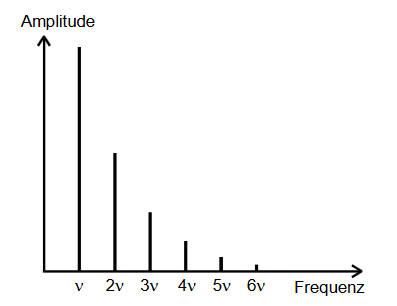
\includegraphics[width=\textwidth-20em]{content/lspek.png}
\end{figure}
\noindent
Aus Abbildung \ref{fig:lspek} ist zu entnehmen, dass die Amplituden $a_n$ und $b_n$ für $n\rightarrow\infty$ gegen Null gehen.


\subsection{Die Fourier-Trnasformation}
Die Fouriertransformation ermöglicht es das gesamte Frequenzspektrum einer zeitlich Funktion zu bestimmen.
Die Fouriertransformation besitzt die Form:
\begin{equation}
  g(\nu)=\int_{-\infty}^{\infty}f(t)e^{i\nu t} dt
\end{equation}
Wenn $f(t)$ periodisch ist, dann setzt sich $g(\mu)$ aus konvergierenden Reihen von $\delta$-Distributionen zusammen.
Zusätzlich ist es möglich aus dem Frequenzspektrum, also der Fouriertransformierten, wieder die Signalfunktion in abhängigkeit von der Zeit zu berechnen.
Die Rücktransformation besitzt die Form:
\begin{equation}
  f(t)= \frac{1}{2\pi}\int_{-\infty}^{\infty} g(\nu) e^{i\mu t} d\nu
\end{equation}
Da es in der Praxis nicht möglich ist über einen unendlich langen Zeitraum zu integrieren, treten Abweichungen von den zu erwartenen Ergebnissen auf.
